\documentclass{standalone}

\usepackage{tikz}

\usetikzlibrary{positioning, chains, shapes.geometric, fit, shapes, arrows.meta, calc}

\begin{document}

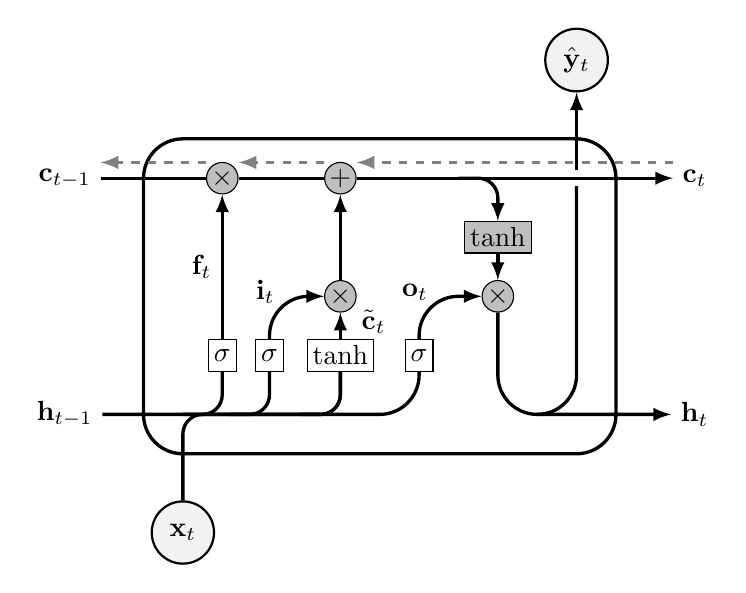
\begin{tikzpicture}[
    >=LaTeX, % Use default LaTeX arrows
    % Styles 
    cell/.style={ % RNN cell
        rectangle, 
        rounded corners=5mm, 
        draw,
        very thick,
        minimum height=4cm,
        minimum width=6cm
    }, 
    cellc/.style={ % RNN cells in a chain
        cell,
        on chain,
        join
    },
    input/.style={ % Input or output node
        circle,
        minimum width=2.25em,
        draw,
        fill=gray!10,
        thick
    },
    hidden/.style={ % Hidden state
    },
    func/.style={ % Functions
        rectangle,
        draw,
        inner sep=2pt,
        minimum height=0.4cm
    },
    op/.style={ % Operators
        circle,
        draw,
        inner sep=-0.5pt,
        minimum height=0.4cm,
    },
    pointwise/.style={ % Pointwise operations and functions
        fill=gray!50,
    },
    arrow/.style={
        -latex,
        very thick
    },
    arrowc1/.style={ % Arrows with rounded corners
        arrow,
        rounded corners=.25cm
    },
    arrowc2/.style={ % Arrows with big rounded corners
        arrow,
        rounded corners=.5cm
    },
    backprop/.style={ % Backpropagation arrows
        arrow,
        dashed,
        gray
    }
]
  
    % LSTM cell
    \node [cell] at (0,0){};

    % Internal functions and operators
    \node [func] (sigf) at (-2,-0.75) {$\sigma$};
    \node [func] (sigi) at (-1.4,-0.75) {$\sigma$};
    \node [func] (tanhi) at (-0.5,-0.75) {$\tanh$};
    \node [func] (sigo) at (0.5,-0.75) {$\sigma$};
    \node [func, pointwise] (tanho) at (1.5,0.75) {$\tanh$};
    \node [op, pointwise] (mulf) at (-2,1.5) {$\times$};
    \node [op, pointwise] (add) at (-0.5,1.5) {+};
    \node [op, pointwise] (muli) at (-0.5,0) {$\times$};
    \node [op, pointwise] (mulo) at (1.5,0) {$\times$};

    % Inputs, outputs and hidden states
    \node[hidden] (ct-1) at (-4,1.5) {$\mathbf{c}_{t-1}$};
    \node[hidden] (ht-1) at (-4,-1.5) {$\mathbf{h}_{t-1}$};
    \node[input] (x) at (-2.5,-3) {$\mathbf{x}_{t}$};
    \node[hidden] (ct) at (4,1.5) {$\mathbf{c}_{t}$};
    \node[hidden] (ht) at (4,-1.5) {$\mathbf{h}_{t}$};
    \node[input] (y) at (2.5,3) {$\hat{\mathbf{y}}_{t}$};

    % Arrows from input and previous hidden states h_{t-1} and c_{t-1}
    \draw [arrowc1, -] (x) -- (x |- ht-1) -| (tanhi);
    \draw [arrowc2, -] (ht-1) -| (sigo);
    \draw [arrowc1, -] (ht-1 -| sigf)++(-0.5,0) -| (sigf); 
    \draw [arrowc1, -] (ht-1 -| sigi)++(-0.5,0) -| (sigi);
    \draw [arrowc1, -] (ht-1 -| tanhi)++(-0.5,0) -| (tanhi);
    \draw [arrow] (ct-1) -- (mulf) -- (add) -- (ct);

    % Arrows for operation flow within LSTM gates
    \draw [arrow] (sigf) -- node[midway, left] {$\mathbf{f}_t$} (mulf);
    \draw [arrowc2] (sigi) |- node[midway, xshift=-1.5, yshift=1.5] {$\mathbf{i}_t$} (muli);
    \draw [arrow] (tanhi) -- node[midway, xshift=12, yshift=1.5] {$\tilde{\mathbf{c}}_t$} (muli);
    \draw [arrowc2] (sigo) |- node[midway, xshift=-1.5, yshift=1.5] {$\mathbf{o}_t$} (mulo);
    \draw [arrow] (muli) -- (add);
    \draw [arrowc1] (add -| tanho) ++(-0.5,0) -| (tanho);
    \draw [arrow] (tanho) -- (mulo);

    % Arrows to output and current hidden states h_t
    \draw [arrowc2] (mulo) |- (ht);
    \draw (ct -| y) ++(0,-0.1) coordinate (i1);
    \draw [arrowc2, -] (ht -| y) ++(-0.5,0) -| (i1);
    \draw [arrow] (i1) ++(0,0.2) -- (y);

    % Backpropagation arrows
    \draw [backprop] ($(ct.west)+(0,0.2)$) -- ($(add.east)+(0,0.2)$);
    \draw [backprop] ($(add.west)+(0,0.2)$) -- ($(mulf.east)+(0,0.2)$);
    \draw [backprop] ($(mulf.west)+(0,0.2)$) -- ($(ct-1.east)+(0,0.2)$);
\end{tikzpicture}

\end{document}